\title{CS 613 - Machine Learning}
\author{
        Assignment 3 - Classification \\
        Robert Thompson \\
}
\date{}
\documentclass[12pt]{article}
\usepackage[margin=0.7in]{geometry}
\usepackage{graphicx}
\usepackage{float}
\usepackage{comment}
\usepackage{amsmath}

\includecomment{versionB}
%\excludecomment{versionB}

\begin{document}
\maketitle

\section{Theory}
\begin{enumerate}
\item Consider the following set of training examples for an unknown target function:  $(x_1, x_2)\rightarrow y$:
\begin{table}[h]
\begin{center}
\begin{tabular}{|l|l|l|l|}
\hline
Y & $x_1$ & $x_2$ & Count\\
\hline
+ & T & T & 3\\
+ & T & F & 4\\
+ & F & T & 4\\
+ & F & F & 1\\
- & T & T & 0\\
- & T & F & 1\\
- & F & T & 3\\
- & F & F & 5\\
\hline
\end{tabular}
\end{center}
\end{table}
	
\begin{enumerate}
	\item What is the sample entropy for the class label overall, $H(Y)$ from this training data (using log base 2) (3pts)? \\
	% START: 1A
	\hfill \linebreak 
	Number of Positive Samples: 3 + 4 + 4 + 1 = 12 \\
	Number of Negative Samples: 0 + 1 + 3 + 5 = 9 \\ 
	Total Number of Samples: 12 + 9 = 21 \\
	\begin{equation*}
    	\begin{split}
    	    H(Y) & = H(\frac{positive}{positive+negative},\frac{negative}{positive+negative}) = H(\frac{12}{12+9},\frac{9}{12+9}) \\
    	    & = (\frac{12}{21} * log_2(\frac{12}{21})) + (\frac{9}{21} * log_2(\frac{9}{21})) \\
    	    & = (-0.57 * log_2(0.57)) + (-0.43 * log_2(0.43)) \\
    	    & = (-0.57 * -0.81) + (-0.43 * -1.22) \\
    	    & = (0.46) + (0.52) \\
    	    & = 0.46 + 0.52 \\
    	    & = 0.98 \\
    	\end{split}
	\end{equation*}
	% END: 1A
	\item What are the weighed average entropies for branching on variables $x_1$ and $x_2$ (4pts)?
	% START: 1A
	\begin{enumerate}
	    \item Get the Total Samples = 21
	    \item Get the counts of each class when split on $x_1$
	    \begin{align*}
	        Positive_T &= 3 + 4 = 7 & Positive_F = 4 + 1 = 5 \\
	        Negative_T &= 0 + 1 = 1 & Negative_F = 3 + 5 = 8 \\ 
	        Total_T &= 7 + 1 = 8 & Total_F = 5 + 8 = 13
	    \end{align*}
	    \item Calculate Weighted Average Entropy (or Information Gain) for $x_1$
	    \begin{equation*}
	        \begin{split}
	            IG(x_1) &= \frac{Total_T}{Total_S} * H(\frac{Positive_T}{Total_T},\frac{Negative_T}{Total_T}) + \frac{Total_F}{Total_S} * H(\frac{Positive_F}{Total_F},\frac{Negative_F}{Total_F}) \\
	            &= \frac{8}{21} * H(\frac{7}{8},\frac{1}{8}) + \frac{13}{21} * H(\frac{5}{13},\frac{8}{13}) \\
	            &= \frac{8}{21} * (-\frac{7}{8} * log_{2}(\frac{7}{8}) - \frac{1}{8} * log_{2}(\frac{1}{8})) + \frac{13}{21} * (-\frac{5}{13} * log_{2}(\frac{5}{13}) - \frac{8}{13} * log_{2}(\frac{8}{13})) \\
	            &= 0.38 * ((-0.875 * -0.19) - (0.125 * 0.32)) + 0.62 * ((-0.38 * -1.4)) - (0.62 * -0.69)) \\
	            &= 0.38 * (0.17 + 0.4) + 0.62 * (0.53 + 0.43) \\
	            &= 0.38 * (0.57) + 0.62 * (0.95) \\
	            &= 0.21 + 0.59 = 0.8 \\
	        \end{split}
	    \end{equation*}
	        Information Gain $x_1$ = Total Entropy - Feature Entropy = 0.98 - 0.8 = 0.13
	    \item Get the counts of each class when split on $x_2$
	    \begin{align*}
	        Positive_T &= 3 + 4 = 7 & Positive_F = 4 + 1 = 5 \\
	        Negative_T &= 0 + 3 = 3 & Negative_F = 1 + 5 = 6 \\ 
	        Total_T &= 7 + 3 = 10 & Total_F = 5 + 6 = 11
	    \end{align*}
	    \item Calculate Weighted Average Entropy (or Information Gain) for $x_2$
	    \begin{equation*}
	        \begin{split}
	            IG(x_2) &= \frac{Total_T}{Total_S} * H(\frac{Positive_T}{Total_T},\frac{Negative_T}{Total_T}) + \frac{Total_F}{Total_S} * H(\frac{Positive_F}{Total_F},\frac{Negative_F}{Total_F}) \\
	            &= \frac{10}{21} * H(\frac{7}{10},\frac{3}{10}) + \frac{11}{21} * H(\frac{5}{11},\frac{6}{11}) \\
	            &= \frac{10}{21} * (-\frac{7}{10} * log_{2}(\frac{7}{10}) - \frac{3}{10} * log_{2}(\frac{3}{10})) + \frac{11}{21} * (-\frac{5}{11} * log_{2}(\frac{5}{11}) - \frac{6}{11} * log_{2}(\frac{6}{11})) \\
	            &= 0.48 * ((-0.7 * -0.51) - (0.3 * -1.74)) + 0.52 * ((-0.45 * -1.12)) - (0.54 * -0.89)) \\
	            &= 0.48 * (0.36 + 0.52) + 0.52 * (0.5 + 0.48) \\
	            &= 0.48 * (0.88) + 0.52 * (0.98) \\
	            &= 0.42 + 0.51 = 0.93 \\
	        \end{split}
	    \end{equation*}
	        Information Gain $x_2$ = Total Entropy - Feature Entropy = 0.98 - 0.93 = 0.05
	\end{enumerate}
	\item Draw the decision tree that would be learned by the ID3 algorithm without pruning from this training data. You may use software to draw this or draw it by hand.  But either way the figure should be embedded in your PDF submission. (5pts) \\
	\begin{figure}[H]
        \begin{center}
        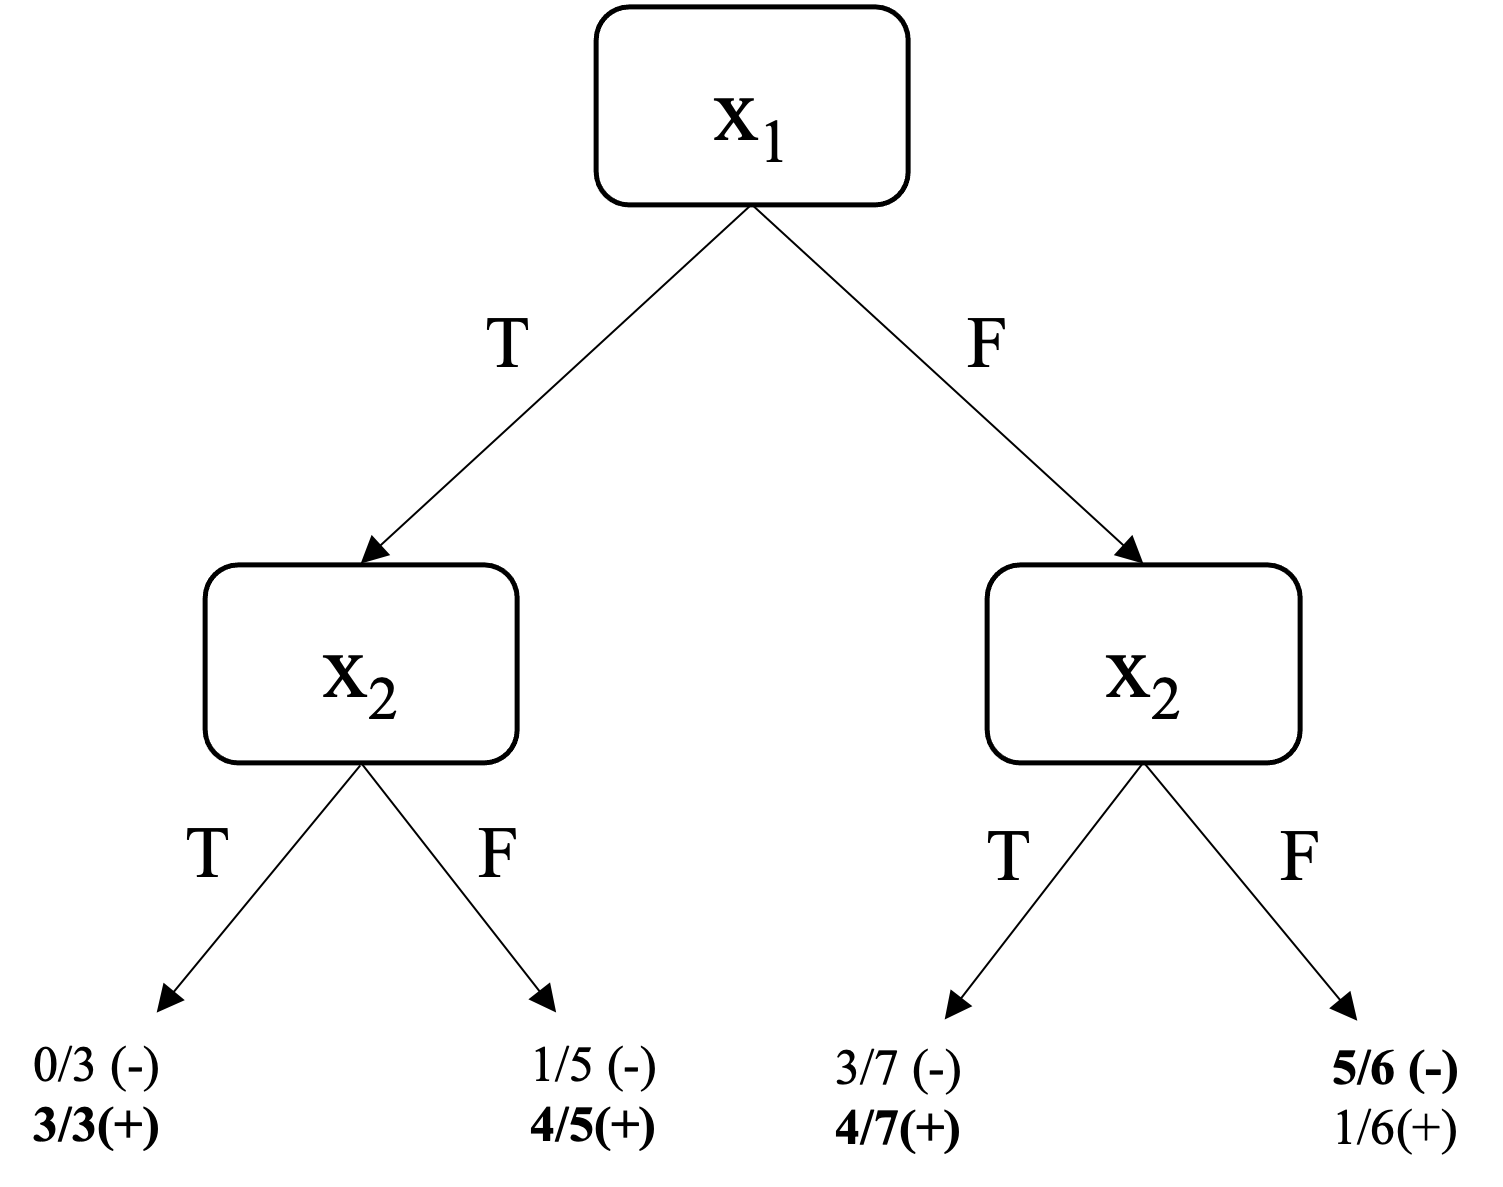
\includegraphics{images/Decision_Tree.png}
        \label{GD}
        \end{center}
    \end{figure}

\end{enumerate}
	
\item We decided that maybe we can use the number of characters and the average word length an essay to determine if the student should get an $A$ in a class or not.  Below are five samples of this data:
\begin{table}[h]
\begin{center}
\begin{tabular}{|l|l|l|}
\hline
\# of Chars & Average Word Length & Give an A\\
\hline
216 & 5.68 & Yes\\
69 & 4.78 & Yes\\
302 & 2.31 & No \\
60 & 3.16 & Yes \\
393 & 4.2 & No\\
\hline
\end{tabular}
\end{center}
\end{table}
	\begin{enumerate}
	\item What are the class priors, $P(A=Yes), P(A=No)$? (3pts) \\
	% START: 2A
	\hfill \linebreak
	Number of Yes Samples = 3 \\
	Number of No Samples = 2 \\ 
	Total Number of Samples: 3 + 2 = 5 \\
	\begin{equation*}
	    P(A = Yes) & = P(\frac{Yes}{Yes+No}) = P(\frac{3}{3+2}) = P(\frac{3}{5}) = 0.6
	\end{equation*}
	\begin{equation*}
	    P(A = No) & = P(\frac{No}{Yes+No}) = P(\frac{2}{3+2}) = P(\frac{2}{5}) = 0.4
	\end{equation*}
	% END: 2A
	\item Find the parameters of the Gaussians necessary to do Gaussian Naive Bayes classification on this decision to give an A or not.  Zscore the features first over all the data together so that there is no unfair bias towards the features of different scales (5pts). \\
	% START: 2B
	\hfill \linebreak
	\begin{enumerate}
	    \item Defines the Training Features
    	 X = 
    	$\begin{bmatrix}
    	   216  & 5.68 \\
    	   69 & 4.78 \\
    	   302 & 2.31 \\
    	   60 & 3.16 \\
    	   393 & 4.2
    	\end{bmatrix}$ \\
	    \item Calculate the Feature Means and Standard Deviations \\ \\
	    $\mu &= \begin{bmatrix} 208 & 4.03 \end{bmatrix} $ \\ 
	    $\sigma &= \begin{bmatrix} 145.22 & 1.33 \end{bmatrix} $ \\
	    \item Z-Score our Training Data
    	\begin{flalign*}
        Features_{zscored}
        &= \begin{bmatrix}
    	   216  & 5.68 \\
    	   69 & 4.78 \\
    	   302 & 2.31 \\
    	   60 & 3.16 \\
    	   393 & 4.2
    	\end{bmatrix} - \begin{bmatrix} 208 & 4.03 \end{bmatrix} / \begin{bmatrix} 145.22 & 1.33 \end{bmatrix} &\\\\ 
    	&= \begin{bmatrix}
    	   0.06  & 1.24 \\
    	   -0.96 & 0.56 \\
    	   0.65 & -1.29 \\
    	   -1.02 & -0.65 \\
    	   1.27 & 0.13
    	\end{bmatrix}
        \end{flalign*}
        \item Calculate the Mean and Standard Deviation for Class "Yes"
    	\begin{flalign*}
        \mu_{feature1} &= \frac{0.06-0.96-1.02}{3} = \frac{-1.92}{3} =-0.64 &&
    	\end{flalign*}
    	\begin{flalign*}
    	\sigma_{feature1} &= \frac{(0.06-(-0.64))^2 + (-0.96-(-0.64))^2 + (-1.02-(-0.64))^2}{3-1} &&\\
    	                    &= \frac{(0.06+0.64)^2 + (-0.96+0.64)^2 + (-1.02+0.64)^2}{2} &&\\
    	                    &= \frac{(0.7)^2 + (-0.32)^2 + (-0.38)^2}{2} &&\\
    	                    &= \frac{(0.49) + (0.1) + (0.14)}{2} &&\\
    	                    &= \frac{0.73}{2} &&\\
    	                    &= 0.37 &&\\
    	\end{flalign*}
    	\begin{flalign*}
        \mu_{feature2} &= \frac{1.24+0.56-0.65}{3} = \frac{1.15}{3} = 0.38 &&
    	\end{flalign*}
    	\begin{flalign*}
    	\sigma_{feature2} &= \frac{(1.24-0.38)^2 + (0.56-0.38)^2 + (-0.65-0.38)^2}{3-1} &&\\
    	                    &= \frac{(0.86)^2 + (0.18)^2 + (-1.03)^2}{2} &&\\
    	                    &= \frac{(0.74) + (0.03) + (1.06)}{2} &&\\
    	                    &= \frac{1.83}{2} &&\\
    	                    &= 0.92 &&\\
    	\end{flalign*}
    	\item Calculate the Mean and Standard Deviation for Class "No"
    	\begin{flalign*}
        \mu_{feature1} &= \frac{0.65+1.27}{2} = \frac{1.92}{2} =0.96 &&
    	\end{flalign*}
    	\begin{flalign*}
    	\sigma_{feature1} &= \frac{(0.65-0.96)^2 + (1.27-0.96)^2}{2-1} &&\\
    	                    &= \frac{(-0.31)^2 + (0.31)^2}{1} &&\\
    	                    &= \frac{(0.1) + (0.1)}{1} &&\\
    	                    &= \frac{0.2}{1} &&\\
    	                    &= 0.2 &&
    	\end{flalign*}
    	\begin{flalign*}
        \mu_{feature2} &= \frac{-1.29+0.13}{2} = \frac{-1.16}{2} = -0.58 &&
    	\end{flalign*}
    	\begin{flalign*}
    	\sigma_{feature2} &= \frac{(-1.29-(-0.58))^2 + (0.13-(-0.58))^2}{2-1} &&\\
    	                    &= \frac{(-1.29+0.58)^2 + (0.13+0.58)^2}{2-1} &&\\
    	                    &= \frac{(-0.71)^2 + (0.71)^2}{1} &&\\
    	                    &= \frac{(0.5) + (0.5)}{1} &&\\
    	                    &= \frac{1}{1} &&\\
    	                    &= 1 &&
    	\end{flalign*}
    	\item Calculated Gaussian Parameters \\\\
    	$\mu_{Y} = \begin{bmatrix} -0.64 & 0.38 \end{bmatrix} $ \\
    	\hfill \linebreak
    	$\sigma_{Y} = \begin{bmatrix} 0.37 & 0.92 \end{bmatrix} $ \\
    	\hfill \linebreak
    	$\mu_{N} = \begin{bmatrix} 0.96 & -0.58 \end{bmatrix} $ \\
    	\hfill \linebreak
    	$\sigma_{N} = \begin{bmatrix} 0.2 & 1 \end{bmatrix} $ \\
	\end{enumerate}
	% END: 2A
	\item Using your response from the prior question, determine if an essay with 242 characters and an average word length of 4.56 should get an A or not.  Show the computations to support your answer. (5pts). \\
    % START: 2C	
	\begin{enumerate}
	    \item Define Validation Features (X) = $\begin{bmatrix}242  & 4.56 \end{bmatrix}$ \\
	    \item Z-Score with Feature Training Data Mean and Standard Deviation:
        \begin{flalign*}
        Features_{zscored}
        &= \begin{bmatrix}242 & 4.56 \end{bmatrix} - \begin{bmatrix}208 & 4.03 \end{bmatrix} / \begin{bmatrix} 145.22 & 1.33 \end{bmatrix} &\\
        &= \begin{bmatrix}(242-208) & (4.56-4.03) \end{bmatrix} / \begin{bmatrix}145.22 & 1.33 \end{bmatrix} & \\
        &= \begin{bmatrix} \frac{34}{145.22} & \frac{0.53}{1.33} \end{bmatrix} & \\
        &= \begin{bmatrix} 0.23 & 0.4 \end{bmatrix}
        \end{flalign*}
        \item Determine if an essay with 242 characters and an average word length of 4.56 should get an A or not:
        \begin{flalign*}
        P(A = Y | F_1 = 0.23, F_2 = 0.4) &= P(A = Y) \times F_1 = 0.23 \times F_2 = 0.4 & \\
        &= 0.6 \frac{1}{\sigma_{1Y}\sqrt{2\pi}}e^{-\frac{(F_1-\mu_{1Y})^2}{2(\sigma_{1Y})^2}} \frac{1}{\sigma_{2Y}\sqrt{2\pi}}e^{-\frac{(F_2-\mu_{2Y})^2}{2(\sigma_{2Y})^2}} & \\
        &= 0.6 \frac{1}{0.37\sqrt{2\pi}}e^{-\frac{(0.23-(-0.64))^2}{2(0.37)^2}} \frac{1}{0.92\sqrt{2\pi}}e^{-\frac{(0.4-0.38)^2}{2(0.92)^2}} & \\
        &= 0.6 \frac{1}{0.37\sqrt{2\pi}}e^{-\frac{(0.23+0.64)^2}{2(0.37)^2}} \frac{1}{0.92\sqrt{2\pi}}e^{-\frac{(0.4-0.38)^2}{2(0.92)^2}} & \\
        &= 0.6 \frac{1}{0.37\sqrt{2\pi}}e^{-\frac{(0.87)^2}{2(0.1369)}} \frac{1}{0.92\sqrt{2\pi}}e^{-\frac{(0.2)^2}{2(0.8464)}} & \\
        &= 0.6 \frac{1}{0.37(2.51)}e^{-\frac{0.76}{0.27}} \frac{1}{0.92(2.51)}e^{-\frac{0.02}{1.69}} & \\
        &= 0.6 \frac{1}{0.93}(0.05) \frac{1}{2.31}(0.98) & \\
        &= 0.6 \times (1.08 \times 0.05) \times (0.43 \times 0.98) & \\
        &= 0.6 \times 0.54 \times 0.42 & \\
        &= 0.13 \\
        \end{flalign*}
        \item Conclusion - Based on the the validation data input into the Gaussian Probability Density Function, there is a 13\% probability that the essay with 242 characters and an average word length of 4.56 will receive an A.
    \end{enumerate}
    % END: 2C	
	\end{enumerate}
\end{enumerate}


\newpage
\section{Naive Bayes Classifier}\label{naive}

\begin{enumerate}
    \item Validation Statistics
    \begin{itemize}
        \item Precision: $0.655373831775701$
        \item Recall: $0.9739583333333334$
        \item F-Measure: $0.7835195530726258$
        \item Accuracy: $0.7979139504563233$
    \end{itemize}
\end{enumerate}

\section{Decision Trees}\label{naive}

\begin{enumerate}
    \item Validation Statistics
    \begin{itemize}
        \item Precision: $0.8317307692307693$
        \item Recall: $0.9010416666666666$
        \item F-Measure: $0.8650000000000001$
        \item Accuracy: $0.894393741851369$
    \end{itemize}
\end{enumerate}

\section{Additional Evaluation}

\begin{enumerate}
    \item Multi-Class Naive Bayes
    \begin{itemize}
        \item Accuracy: $0.8166431593794076$
    \end{itemize}
    \item Multi-Class Decision Trees
    \begin{itemize}
        \item Accuracy: $0.8998589562764456$
    \end{itemize}
\end{enumerate}

\end{document}